\documentclass[11pt,a4paper]{article}
\usepackage[UTF8]{ctex}
\usepackage[a4paper,left=23mm,right=23mm,top=19mm,bottom=20mm]{geometry}
\usepackage{fontspec,xeCJK,graphicx,booktabs,tabularx,array,amsmath}
\usepackage[hidelinks]{hyperref}
\setmainfont{Times New Roman}
\setCJKmainfont{SimSun}[BoldFont=SimHei]
\setCJKsansfont{SimHei}
\setlength{\parindent}{2em}
\setlength{\parskip}{3pt}
\linespread{1.08}
\setlength{\tabcolsep}{5pt}
\emergencystretch=1em
\pagestyle{plain}
\begin{document}
\section*{数据预处理与探索性分析}
\subsection*{1 数据来源、关联与质量核查}
附件包含土地资源、作物适种信息、2023年种植记录和生产经营参数四类基础资料。它们的记录粒度不同：地块表描述可用土地，种植表记录某地块某季种了什么，参数表则按作物、地类与季次给出统计数值。将这些资料按各自的键关联，才能使一条种植记录对应正确的土地容量和生产条件。\par
{\centering\small 表1 基础资料的结构与用途\par}\nopagebreak\smallskip
\par\noindent{\small\renewcommand{\arraystretch}{1.22}\begin{tabularx}{\linewidth}{>{\raggedright\arraybackslash}X>{\raggedright\arraybackslash}X>{\raggedright\arraybackslash}X>{\raggedright\arraybackslash}X}\toprule
资料 & 记录数量 & 关联字段 & 内容与单位 \\\midrule
附件1地块表 & 54 & 地块名 & 地类、物理面积（亩） \\
附件1作物表 & 41 & 作物编号 & 名称、类别、适种说明 \\
附件2种植表 & 87 & 地块—作物—季次 & 2023年种植面积（亩） \\
附件2统计表 & 107 & 作物—地类—季次 & 亩产（斤/亩）、成本（元/亩）、价格（元/斤） \\
\bottomrule\end{tabularx}}\par\medskip
预处理采用保留原值和来源的方式。地块名称、地类等字段去除首尾空白，合并单元格中的共享标签按其锚点解释，内部换行与适种说明保持原义。核查的69处关键字段空白均属于合并标签省略，其中作物适种说明36处、种植地块标签33处；另有83个单元格含首尾空白。这些情况属于表格表达问题，不是缺失的产量或市场观测。既有规范化字段与来源锚点核对一致，故直接复用，不重复修改基础数据。\par
智慧大棚第一季的18组参数依据附件2附注明文引用普通大棚第一季对应值，分别保留引用对象和源行。87条历史种植记录中，81条直接匹配统计表，6条通过上述规则匹配。按地块—作物—季次检查未发现重复键，合种的不同作物记录分别保留；107条直接参数均通过数值类型和正值检查，价格区间上下界有序。原表与基础表的1704个来源字段核对一致，18组引用参数亦可追溯。因此，本次不进行统计插补、极值删除或数值标准化。\par
{\centering\small 表2 信息类型及处理方式\par}\nopagebreak\smallskip
\par\noindent{\small\renewcommand{\arraystretch}{1.22}\begin{tabularx}{\linewidth}{>{\raggedright\arraybackslash}X>{\raggedright\arraybackslash}X>{\raggedright\arraybackslash}X}\toprule
对象 & 识别结果 & 采用方式 \\\midrule
合并标签与首尾空白 & 可由原表结构定位 & 复用规范化字段，保留原值和锚点 \\
智慧大棚第一季参数 & 有明确引用依据 & 关联普通大棚源参数，不计为新增观测 \\
原价格区间 & 107条区间格式有效 & 保留上下界，不将中点视为实际成交均价 \\
预期销量 & 附件无独立销量记录 & 保留未知，与生产能力信息分开 \\
\bottomrule\end{tabularx}}\par\medskip
统计表注明，其数据为2023年根据近几年相应资料统计所得。因此，下文将107条记录视为不同生产条件下的参数摘要，不作为107次独立随机抽样，也不将18条引用记录重复计入参数分布。既有“种植面积乘统计亩产”形成的产量估计不属于实际销量，本章的描述性分析仅使用来源明确的面积、类别和原统计参数。\par
\newpage
\subsection*{2 土地尺度与历史种植结构}
为区分土地数量与实际资源规模，图1同时展示各地类面积和单地块尺度。54个地块合计1213亩，其中梯田619亩，占51.03\%；普通大棚和智慧大棚共20个，占地块数的37.04\%，但合计仅12亩，占总面积0.99\%。露天地块面积为6—86亩，大棚均为0.6亩。同样增加一个种植地块，对不同地类意味着很不相同的面积变化，管理要求应结合地块尺度表达。\par
\par\noindent\hfil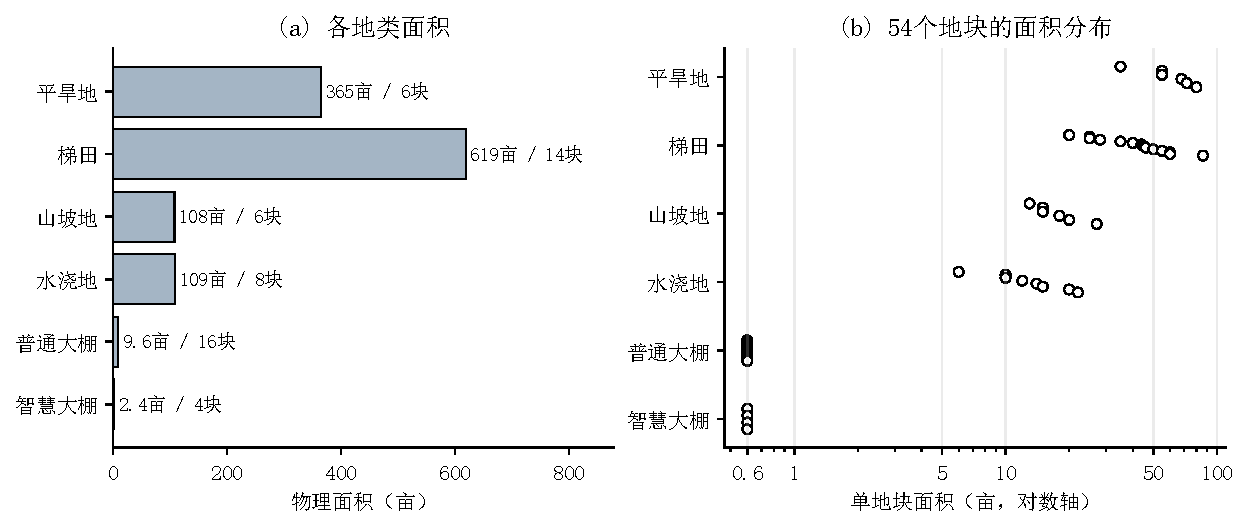
\includegraphics[width=1.0\linewidth]{../../data/eda/DATA-EDA-PAPER-v1/figures_final/01_land.pdf}\hfil\par\nopagebreak
{\centering\small 图1 各地类物理面积与地块尺度。右图每点代表一块地，对数轴用于同时显示大棚和露天地块；纵向错开仅便于辨认。\par}\medskip
历史播种规模按地块—作物—季次记录累计，以亩次表述跨季面积。2023年累计播种面积为1292亩次，其中露天地块1268亩次，大棚24亩次；这与1213亩物理面积的差异来自复种。进一步按地类和作物类别分解，结果见图2。水浇地中，42亩用于单季水稻，其余67亩种植两季蔬菜，形成176亩次；大棚两季累计面积恰为物理面积的两倍。\par
\par\noindent\hfil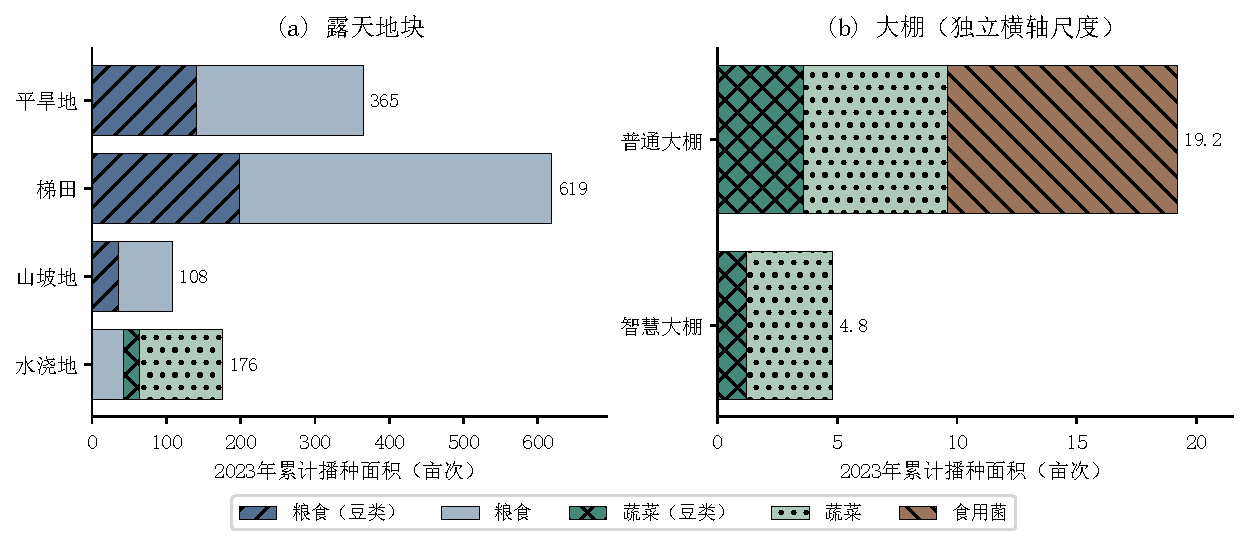
\includegraphics[width=1.0\linewidth]{../../data/eda/DATA-EDA-PAPER-v1/figures_final/03_history_structure.pdf}\hfil\par\nopagebreak
{\centering\small 图2 2023年各地类的播种结构。左右子图采用不同横轴尺度；豆类与同类非豆类分开统计。\par}\medskip
87条记录对应80个地块—季次组，各组种植面积之和均等于对应地块容量，其中7组包含两种作物。豆类累计种植400.8亩次，分布于19个不同地块。上述记录提供了规划起点，但一年内的累计豆类面积不等于三年内所有土地的空间覆盖，历史满种也不自动构成未来必须满种的条件。各作物的播种面积与地块数明细见附图A1。\par
\newpage
\subsection*{3 适种条件与历史观测覆盖}
为判断历史种植是否覆盖全部可选生产条件，按附件适种规则建立作物—地类—季次对应表，并叠加2023年实际记录。图3将“规则不适用”“适种但未记录”和“适种且有记录”分开，避免将没有种植误写为不允许种植。\par
\par\noindent\hfil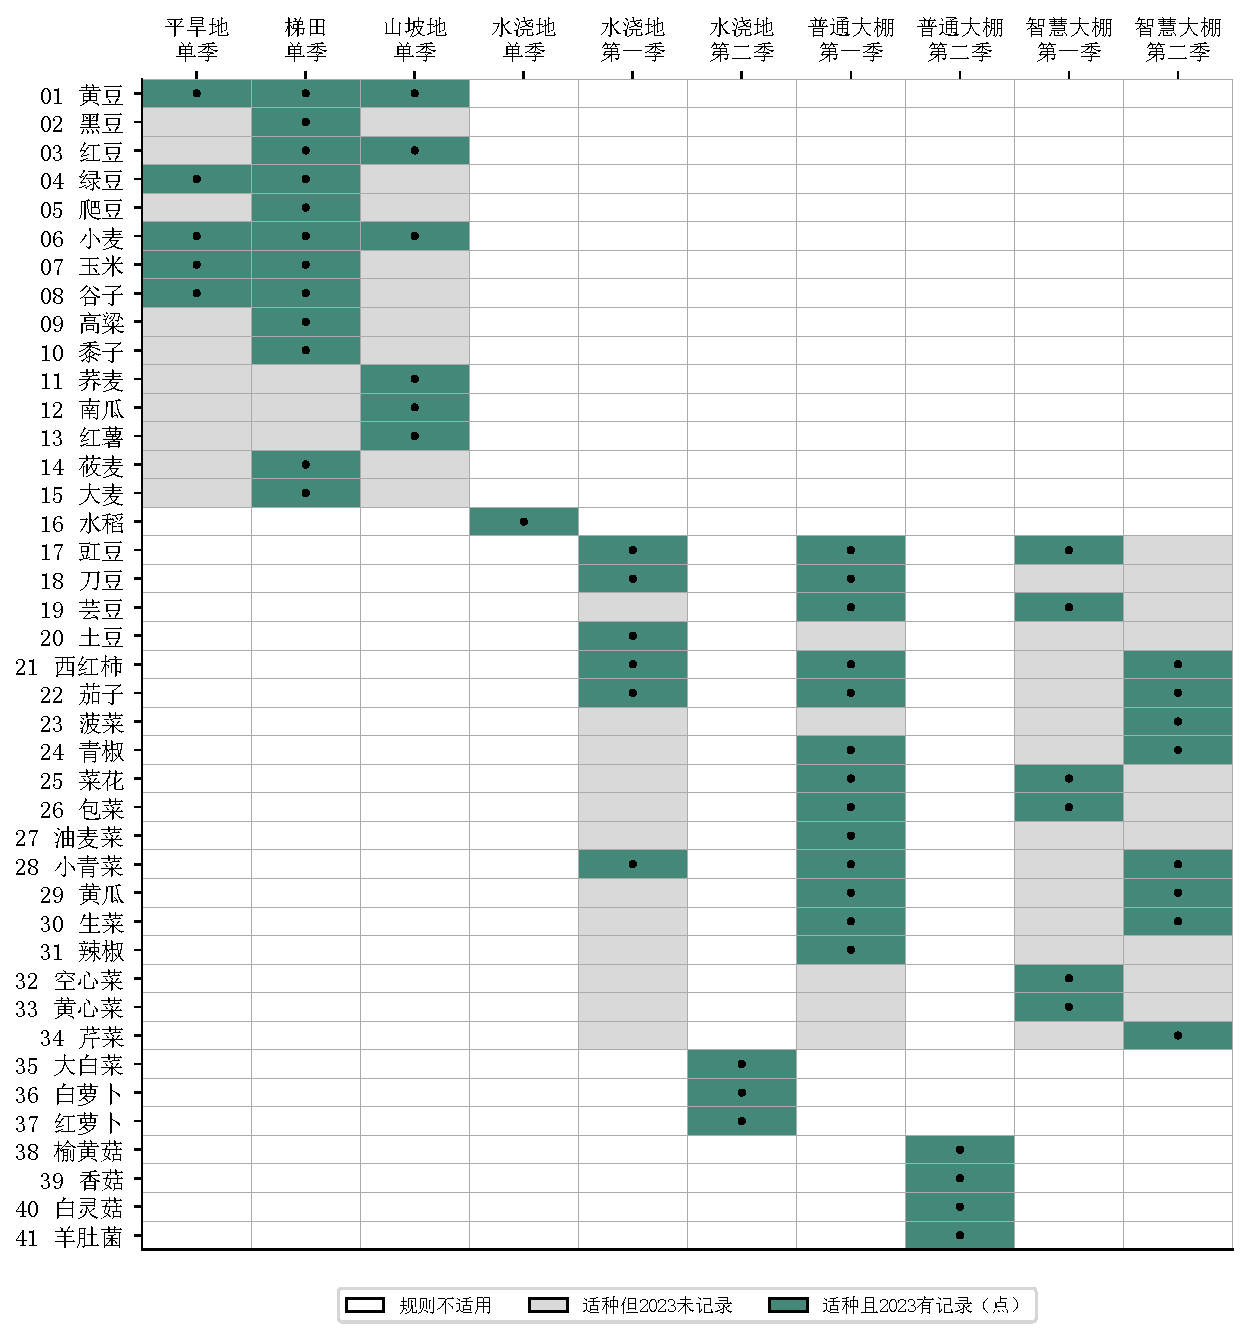
\includegraphics[width=.98\linewidth]{../../data/eda/DATA-EDA-PAPER-v1/figures_final/02_coverage.pdf}\hfil\par\nopagebreak
{\centering\small 图3 作物适种条件与2023年观测覆盖。每格表示一种作物在一种地类、季次下的状态；黑点标记存在种植记录，不表示面积大小或市场需求。\par}\medskip
125个合法组合中，64个有历史种植记录，61个没有。若只保留历史出现过的组合，将遗漏原题允许的生产选择。按作物与模板季次合并后，59个合法组合中仍有12个未观测到种植，这与上述61个缺口的统计粒度不同。因此，适种集合应来自附件规则，历史表用于表达基期安排；二者不宜互相替代。图中的状态也不提供正常销售量或实际销售时段的信息。\par
\newpage
\subsection*{4 生产经营参数的差异与使用口径}
图4在统一坐标尺度下比较粮食、蔬菜和食用菌的亩产与亩成本。不同类别的参数跨度较大：粮食类成本为350—2000元/亩，蔬菜类为500—5500元/亩，食用菌为2000—10000元/亩。图中采用对数坐标以保留全部数值，没有因跨类别差异删除记录；参数点的分布用于认识生产条件，不用于估计经验概率或因果关系。\par
\par\noindent\hfil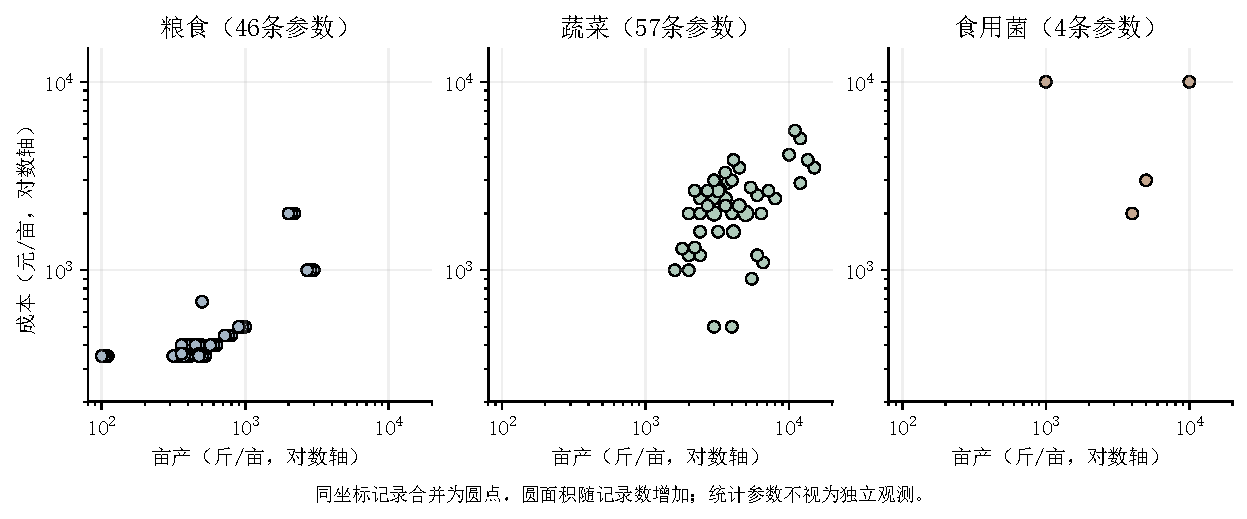
\includegraphics[width=1.0\linewidth]{../../data/eda/DATA-EDA-PAPER-v1/figures_final/04_yield_cost.pdf}\hfil\par\nopagebreak
{\centering\small 图4 107条直接统计参数的亩产与成本分布。粮食、蔬菜分别包含其豆类；同坐标记录合并显示，18条明文引用参数不重复计入。\par}\medskip
同作物比较能进一步区分地类差异与品种差异。15种非水稻粮食作物的统计亩产均呈平旱地高于梯田、梯田高于山坡地的顺序，而各作物在三类土地上的亩成本和价格区间相同。例如，小麦亩产分别为800、760和720斤/亩，成本均为450元/亩，价格区间均为3—4元/斤。因此，采用一个跨地类平均亩产会抹去附件给出的生产差别，参数关联应保留地类维度；该差别属于题给摘要，不能解释为控制其他因素后的因果效应。\par
价格同样应与作物和生产季次匹配。附图A2保留了107条原记录中按作物去除重复后的59组价格区间，其中18种蔬菜在智慧大棚第二季具有单独区间。食用菌的价格跨度尤为明显：白灵菇为14—18元/斤，羊肚菌为80—120元/斤；两者亩成本均为10000元，亩产分别为10000和1000斤。价格高并不意味着单位土地收益必然更高，收入还取决于产量、正常销售量和超额处置方式。因此，本章保留价格区间，不据单价或亩产排列最优作物。\par
{\centering\small 表3 不同设施的通常种植时段\par}\nopagebreak\smallskip
\par\noindent{\small\renewcommand{\arraystretch}{1.22}\begin{tabularx}{\linewidth}{>{\raggedright\arraybackslash}X>{\raggedright\arraybackslash}X>{\raggedright\arraybackslash}X}\toprule
土地类型 & 第一季 & 第二季 \\\midrule
水浇地（双季） & 3—6月前后 & 7—10月前后 \\
普通大棚 & 5—9月前后 & 9月至次年4月前后 \\
智慧大棚 & 3—7月前后 & 8月至次年2月前后 \\
\bottomrule\end{tabularx}}\par\medskip
表3表明，相同季次标签并不对应完全相同的月份。结果模板以2024—2030年为年度位置，单季填第一季；这一填表规则不自动确定跨年收入归属或不同设施共享的销量池。数据能够支持土地规模、生产适配和基期种植结构的描述，市场需求与跨期决策则应采用明确且一致的建模口径。由此形成的输入基础保留了资源差异、历史接续和价格区间，供后文分别组织农业约束与销售收益关系。\par
\newpage
\section*{附录：探索性分析明细}
\subsection*{A1 各作物的历史播种规模与地块分布}
下图完整列出41种作物。小麦累计种植222亩次、涉及4块地；羊肚菌仅4.2亩次、涉及7个大棚。这说明播种面积与地块数量反映不同的管理尺度；地块数本身不表示地块间距离。\par
\par\noindent\hfil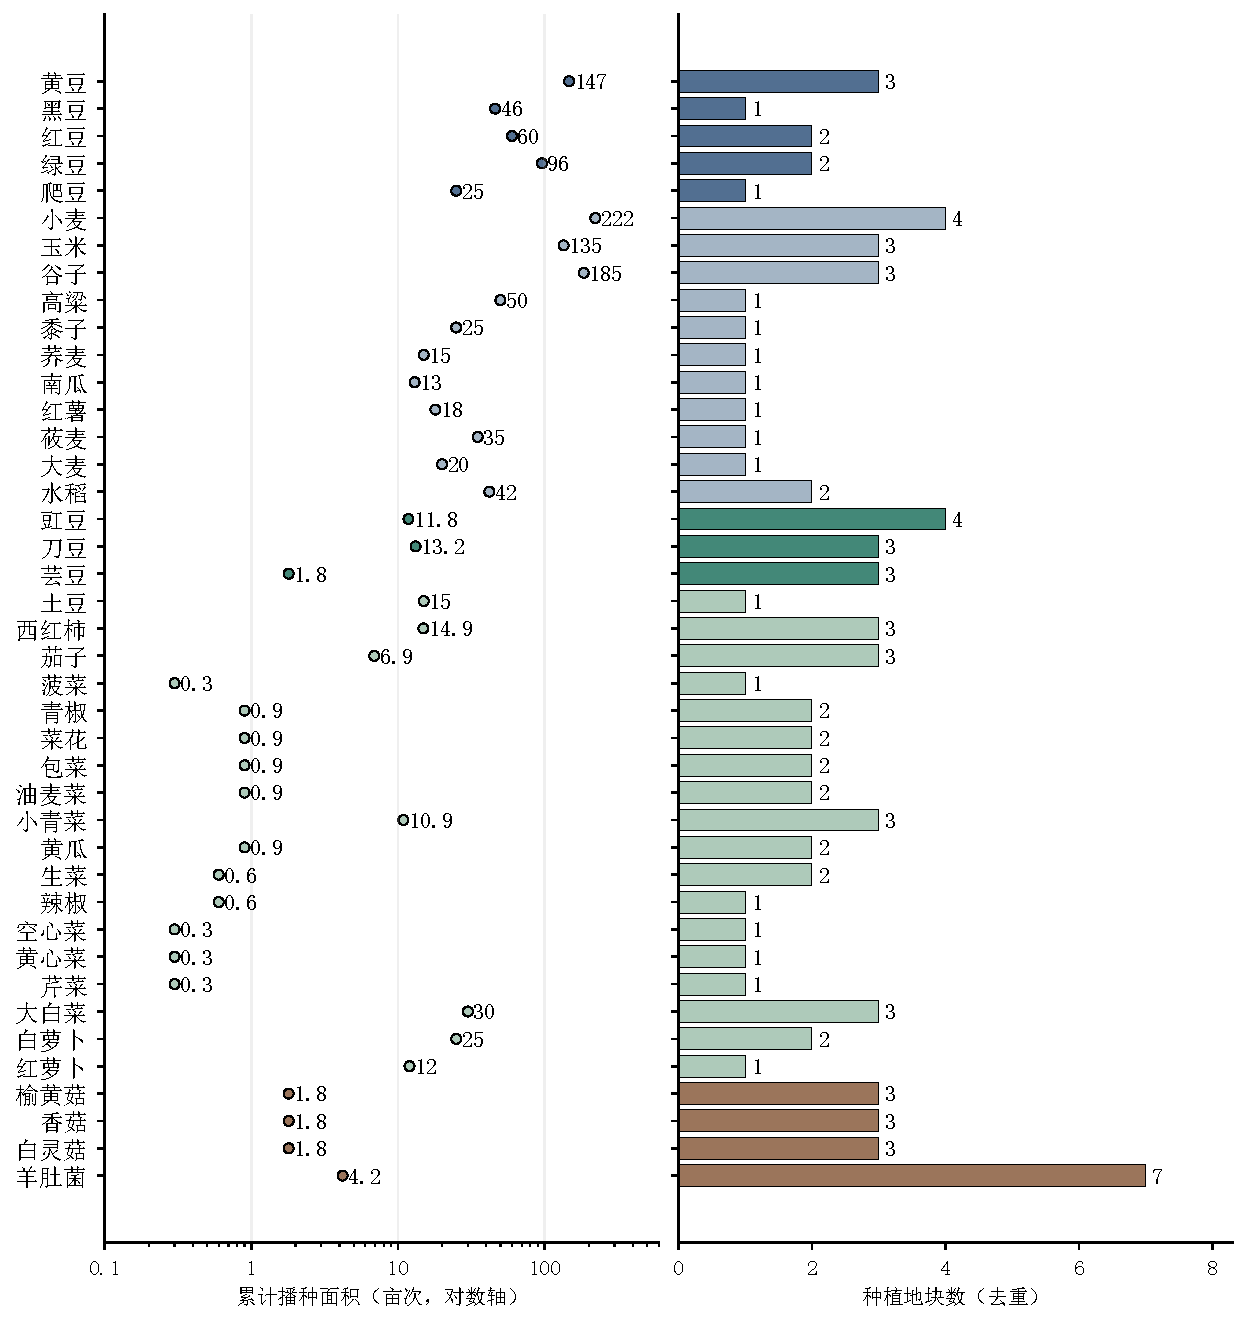
\includegraphics[width=.98\linewidth]{../../data/eda/DATA-EDA-PAPER-v1/figures_final/05_crop_history.pdf}\hfil\par\nopagebreak
{\centering\small 附图A1 2023年各作物累计播种面积与去重地块数。左侧对数轴用于显示0.3—222亩次的全部记录；右侧同一作物跨季重复使用同一地块时只计一次。\par}\medskip
\newpage
\subsection*{A2 原始价格区间}
下图保留各作物的原区间端点。同一作物、不同地类或季次具有相同区间时合并显示，原记录来源仍分别保留；智慧大棚第二季用虚线和圆点区分。这里的区间不是置信区间，也不代表各价格出现的概率。\par
\par\noindent\hfil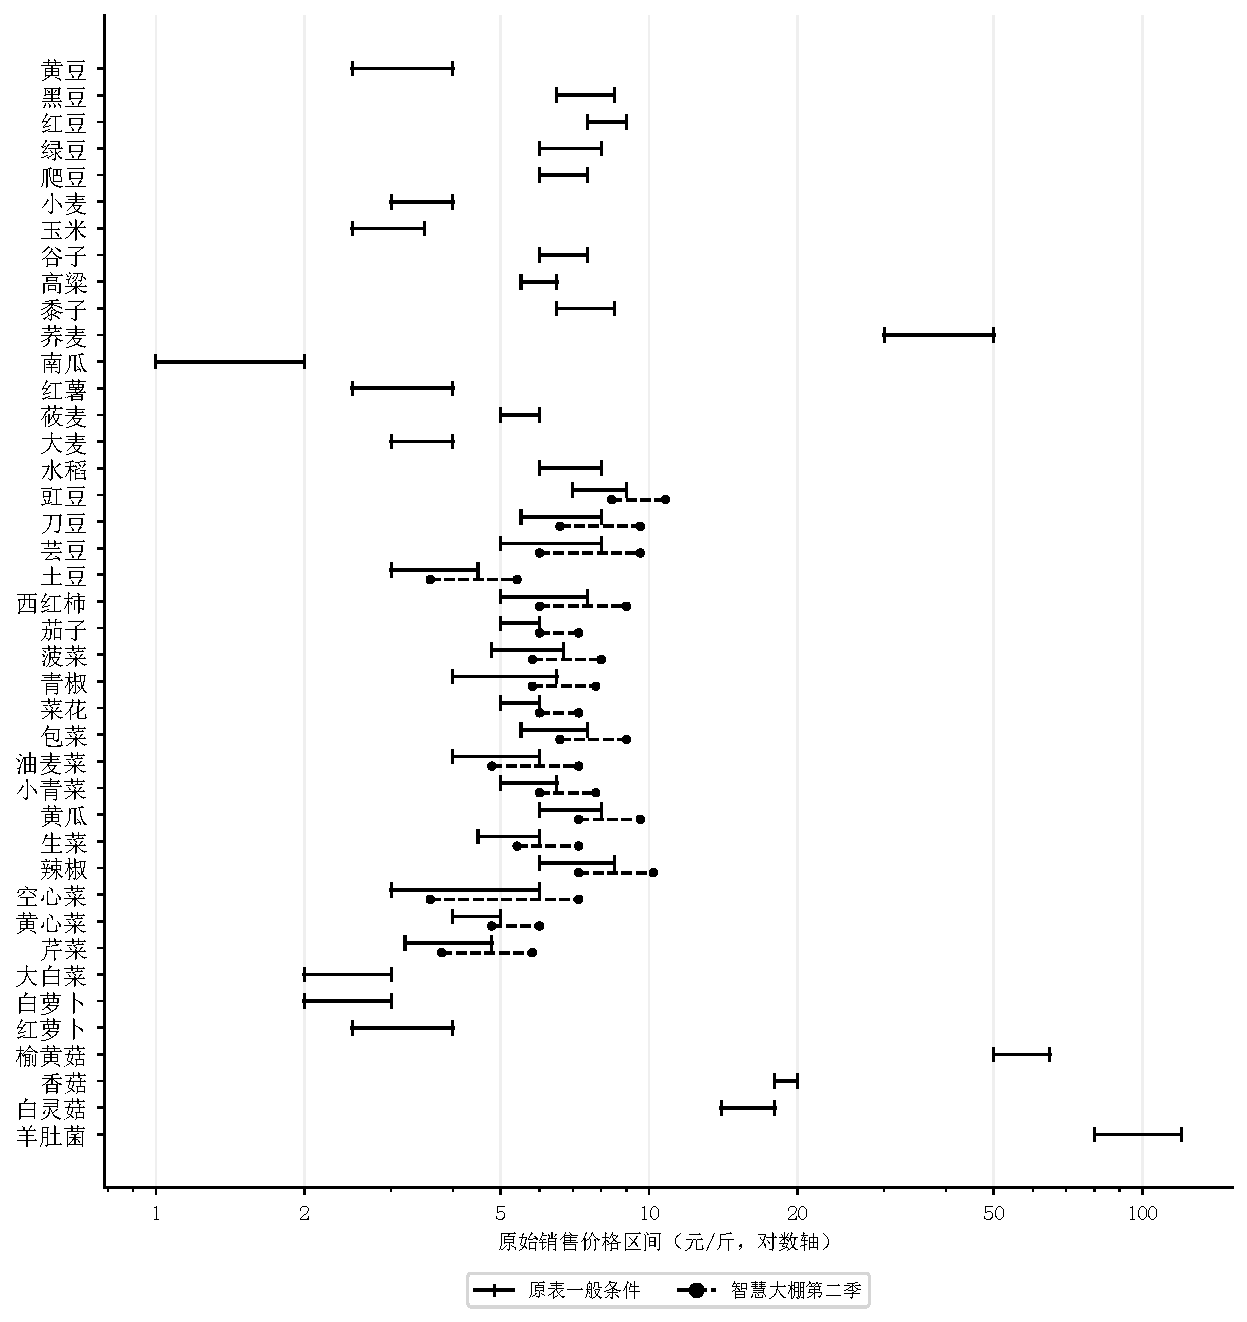
\includegraphics[width=.98\linewidth]{../../data/eda/DATA-EDA-PAPER-v1/figures_final/06_price_intervals.pdf}\hfil\par\nopagebreak
{\centering\small 附图A2 各作物原始销售价格区间。横轴为对数尺度，同作物的不同条件分行显示；没有取价格中点，也没有对不同作物进行平均。\par}\medskip
\end{document}